\documentclass{article}

\usepackage{geometry}
\geometry{a4paper, margin=1in}
\usepackage{graphicx}
\usepackage{listings}
\usepackage{float}
\usepackage{xcolor}
\usepackage[utf8]{inputenc}

\lstset{
    basicstyle=\ttfamily\small,
    breaklines=true,
    frame=single,
    language=C,
    keywordstyle=\color{blue},
    commentstyle=\color{green!50!black},
    stringstyle=\color{red}
}

\begin{document}

\title{Operating Systems Lab Assignment: Synchronization and Scheduling}
\author{Kendyn Fredieu}
\date{October 23, 2025}
\maketitle

\section{Introduction}
This report documents the implementations and analyses for the synchronization and scheduling lab assignment, covering five provided problems and four additional exercises using mutexes and condition variables.

\section{Exercise 1: Hello World}
\lstinputlisting{hello_world.c}
\textbf{Explanation}: Explain why the original code fails and how mutexes and condition variables fix it.\\
\textbf{Analysis}: Discuss synchronization behavior.\\
\textbf{Screenshot}: Include a screenshot of compiling and running hello\_world.c.
\begin{figure}[H]
    \centering
    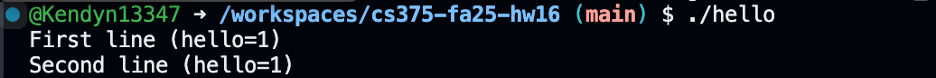
\includegraphics[width=\textwidth]{hello_world.png}
    \caption{Compilation and execution of hello\_world.c}
\end{figure}

\section{Exercise 2: SpaceX Problems}
\lstinputlisting{spacex.c}
\textbf{Explanation}: Describe the original issue and the synchronization fix.\\
\textbf{Analysis}: Analyze countdown and announcement behavior.\\
\textbf{Screenshot}: Include a screenshot of compiling and running spacex.c.
\begin{figure}[H]
    \centering
    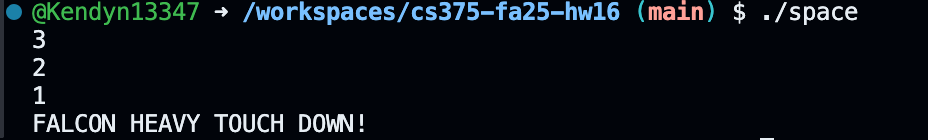
\includegraphics[width=\textwidth]{spacex.png}
    \caption{Compilation and execution of spacex.c}
\end{figure}

\section{Exercise 3: I Love You, Unconditionally!}
\lstinputlisting{love.c}
\textbf{Explanation}: Explain how condition variables ensure correct output.\\
\textbf{Analysis}: Discuss race condition prevention.\\
\textbf{Screenshot}: Include a screenshot of compiling and running love.c.
\begin{figure}[H]
    \centering
    
\includegraphics[width=\textwidth]{love.png}
    \caption{Compilation and execution of love.c}
\end{figure}

\section{Exercise 4: Locking Up the Floopies}
\lstinputlisting{floopy.c}
\textbf{Explanation}: Describe the deadlock issue and lock ordering solution.\\
\textbf{Analysis}: Provide a deadlock scenario and analyze the fix.\\
\textbf{Screenshot}: Include a screenshot of compiling and running floopy.c.
\begin{figure}[H]
    \centering
    
\includegraphics[width=\textwidth]{floopy.png}
    \caption{Compilation and execution of floopy.c}
\end{figure}

\section{Exercise 5: Baking with Condition Variables}
\lstinputlisting{baking.c}
\textbf{Explanation}: Explain how condition variables coordinate baking steps.\\
\textbf{Analysis}: Discuss thread synchronization.\\
\textbf{Screenshot}: Include a screenshot of compiling and running baking.c.
\begin{figure}[h]
    \centering
    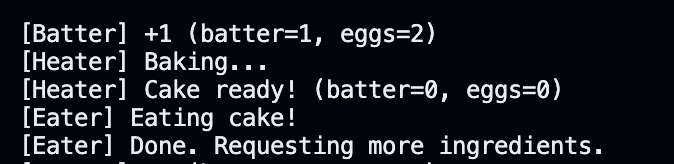
\includegraphics[width=\textwidth]{baking.png}
    \caption{Compilation and execution of baking.c}
\end{figure}

\section{Exercise 6: Priority Donation in Transfer}
\lstinputlisting{priority_transfer.c}
\textbf{Explanation}: Describe how priority donation prevents priority inversion.\\
\textbf{Analysis}: Analyze priority handling.\\
\textbf{Screenshot}: Include a screenshot of compiling and running priority\_transfer.c.
\begin{figure}[H]
    \centering
    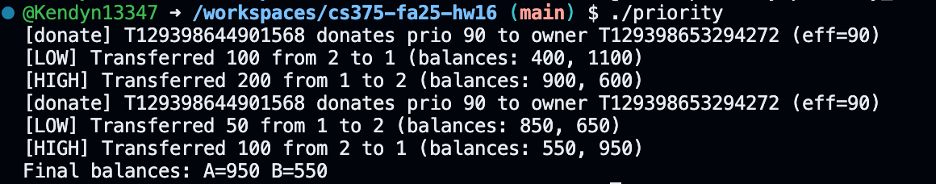
\includegraphics[width=\textwidth]{priority.png}
    \caption{Compilation and execution of priority\_transfer.c}
\end{figure}

\section{Exercise 7: Barrier Synchronization}
\lstinputlisting{barrier.c}
\textbf{Explanation}: Explain how the barrier synchronizes threads.\\
\textbf{Analysis}: Discuss barrier behavior.\\
\textbf{Screenshot}: Include a screenshot of compiling and running barrier.c.
\begin{figure}[H]
    \centering
    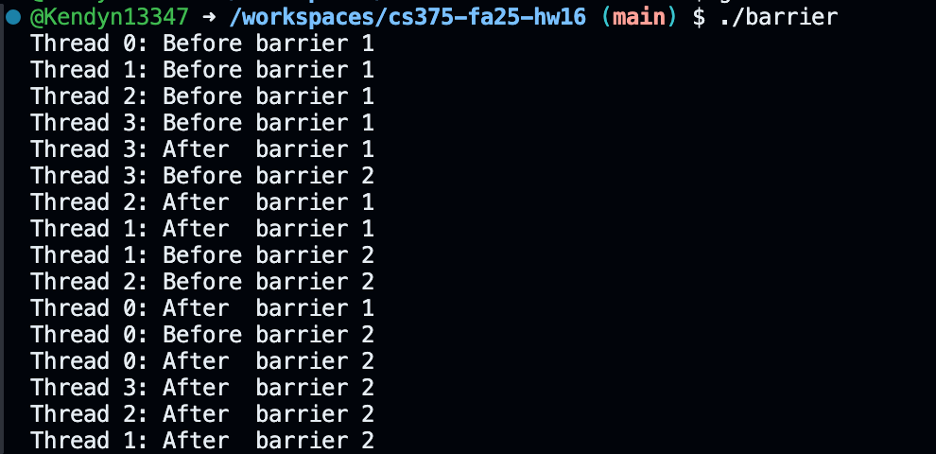
\includegraphics[width=\textwidth]{barrier.png}
    \caption{Compilation and execution of barrier.c}
\end{figure}

\section{Exercise 8: Readers-Writers with Priority}
\lstinputlisting{readers_writers.c}
\textbf{Explanation}: Describe writer priority enforcement.\\
\textbf{Analysis}: Analyze reader-writer interactions.\\
\textbf{Screenshot}: Include a screenshot of compiling and running readers\_writers.c.
\begin{figure}[H]
    \centering
    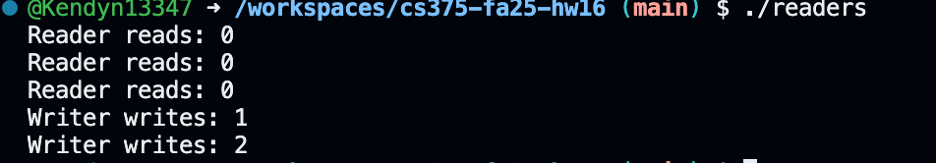
\includegraphics[width=\textwidth]{readers.png}
    \caption{Compilation and execution of readers\_writers.c}
\end{figure}

\section{Exercise 9: Thread Pool}
\lstinputlisting{thread_pool.c}
\textbf{Explanation}: Explain how the thread pool uses a thread-safe queue.\\
\textbf{Analysis}: Discuss efficiency benefits.\\
\textbf{Screenshot}: Include a screenshot of compiling and running thread\_pool.c.
\begin{figure}[H]
    \centering
    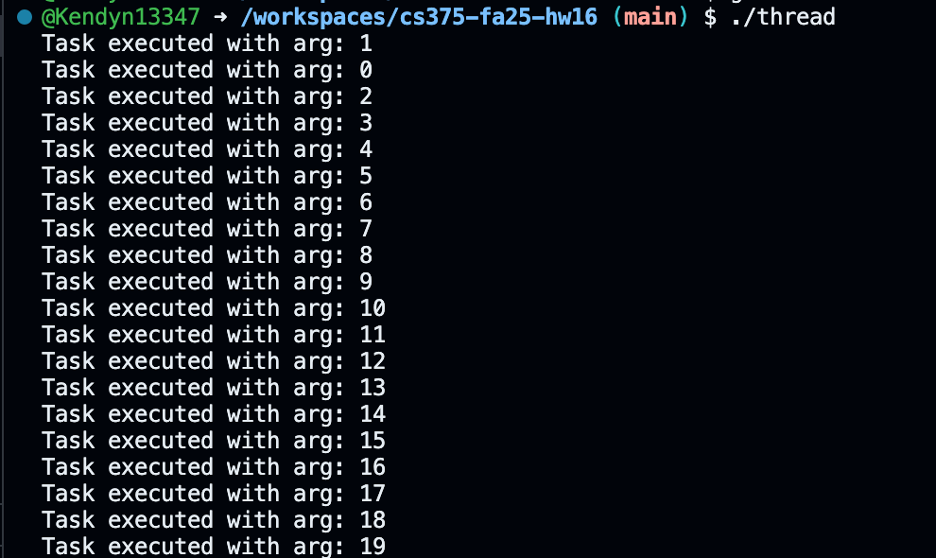
\includegraphics[width=\textwidth]{thread_pool.png}
    \caption{Compilation and execution of thread\_pool.c}
\end{figure}

\end{document}
